\section{Support Vector Machines}

	\paragraph{Motivation and Background}
\begin{sectionbox}

	\subsection{Kernel Methods} 
	Kernel Methods is non-parametic estimation, these make no assumption on statistical model $\rightarrow$ purely Data-Based. \\
	\textbf{Test Statistic} 
	$\boxed{\mathbb{X} \rightarrow \mathbb{R}, \mathbf{x}\mapsto S(\mathbf{x})= \sum_{k=1}^{M} \lambda_kg(\mathbf{x}, \mathbf{\mu_k})}$ \\
	linear combination of Kernel Function $g(.,\mu_k)$, g() generally non-linear pos. definite \\ %TODO: besser einrichten
	
	$\mu_k$: representative for Sample Set $\mathbb{S}=\{x_1,...,x_M\}$ \\  
	$\lambda_k$: weight coefficient determined by learning \\
	Sample Set $\mathbb{S}$ is Empirical Characterization of Unknown Statistical Model \\
	Infernce of $\lambda_k$ based on Sample Set or Training Set is called \textbf{Learning}

	
\end{sectionbox}

\begin{sectionbox}
	\subsection{Kernel Tests}
Statistical Hypothesis Test, where a Sufficient Test Statistic is compared to threshold(i.e.R(x)$\geq$c) decomposes sample space $\mathbb{X}$ into two disjoint subsets$(\mathbb{X}=\mathbb{X}_0\cup\mathbb{X}_1)$ \\
Seperating surface between $\mathbb{X}_0$ and $\mathbb{X}_1$ given by:\\
$\{\mathbf{x}|R(\mathbf{x})=c\}$
The relative postion of a sample $x_j$ to the seperating surface determines choice of hypothesis\\
$\boxed{\mathbb{S} = \{(x_1, y_1),...,(x_M, y_M)\}}$ %TODO: Einrichten
\\
$x_i \in \mathbb{R}^N$, $y_i \in \{\Theta_0, \Theta_1\}$ \\
Inference of Hypothesis Test based on a Sample Set that includes Labeling $y_i$ of the elements $x_i$ is called \textbf{Supervised Learning} \\
Size M of samples has to statisfy:
$\boxed{M \geq dim(\mathbb{X})}$ \\
Because underlying statistical model is unknown, true $\theta_{0}$ and $\theta_{1}$ irrelevant $\rightarrow$ replace them by e.g. {-1,+1} for decision between hypotheses
\end{sectionbox}


\begin{sectionbox}
\subsection{Linear Kernels}
\textbf{Test Statistic} for linear test \\
$\boxed{S(x) = \sum_{i = 1}^{M}\lambda_i\mathbf{x_i}^T\mathbf{x} + wo = \mathbf{w}^T\mathbf{x} +wo}$ $\mathbf{w} = \sum_{i = 1}^{M}\lambda_ix_i$ \\
Hyperplane defined by $\mathbf{w}$(normal vector or weight vector) and $w_o$\\ approximates seperating surface between $\mathbb{X_-}$ and $\mathbb{X_+} \\\rightarrow$Decistion rule T(x):\\
$\boxed{T(\mathbf{x}) = sign(S(\mathbf{x})) = \begin{cases} 
			+1&;\quad \mathbf{w}^T\mathbf{x} +wo \geq 0\\
	        -1&;\quad otherwise
	\end{cases}}$\\ 

\parbox{5.5cm}{\emph{Linear Kernel Test in sample space $\mathbb{X}$:} \\
	(Orientation of w chosen such that w points into direction of $\theta_{1}$("+1"hypothesis)) \\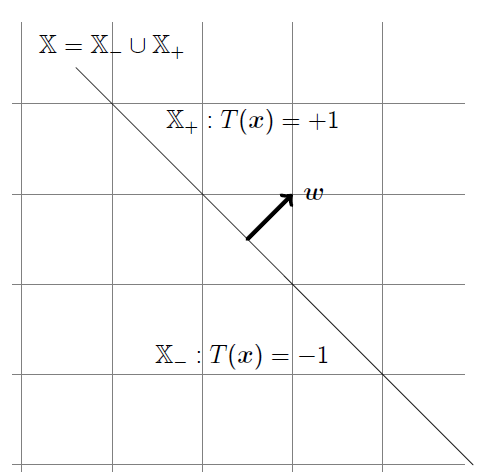
\includegraphics[width = 3cm,height=2.5cm]{linearkerneltest}}%original w=5,H=4


To determine $\mathbf{w}$ and $w_0$ formulate problem as constrained optimaization problem with the constraints: \\
$\forall k\in \{1,...M\}:T(\mathbf{x}_k)= y_k$ \\
$\Rightarrow$ \textbf{Support Vector Methods}:$\boxed{y_k(\mathbf{w}^T\mathbf{x}_k+wo)\geq \epsilon, \forall k}$ \begin{flushright}Robust solution: maximize margin $\epsilon$ for constant norm of $\mathbf{w}$ \end{flushright} 

\end{sectionbox}

\paragraph{Application}
\begin{sectionbox}
	
\subsection{Support Vector Methods}
only feasible for normalized weight vectors \\
%{0 \leq q \leq n-1}} f(q) \le n$,
$\smash{\displaystyle\max_{w}}$ $\epsilon$  s.t.  $y_k \frac{\mathbf{w}^T}{\norm{\mathbf{w}}_2}\mathbf{x}_k \geq \epsilon, \forall k$ , $w_0 = 0$\\ 
$\Leftrightarrow$\hspace{1pt} $\smash{\displaystyle\min_{w}}$ $\frac{1}{2}\norm{\mathbf{w}}_{2}^{2}$ s.t. $y_k\mathbf{w}^T\mathbf{x}_k \geq1, \forall k$ \\
Optimization Problem convex $\rightarrow$ \textbf{Langragian Method} \\ \\
Dual Problem: $\smash{\displaystyle\max_{\mathbf{u}}}$$\smash{\displaystyle\min_{\mathbf{w}}}$ $\Phi (\mathbf{w}, \mathbf{u})$ s.t. $\mathbf{u} \geq 0$ \\ \\
Langragian Multiplier: $u_k \geq 0$   \\
Langragian Fct: $\Phi (\mathbf{w}, \mathbf{u}) = \frac{1}{2}\mathbf{w}^T\mathbf{w} +\sum_{k=1}^{M}u_k(1-y_k\mathbf{w}^T\mathbf{x_k})$  \\
$\frac{\partial\Phi (\mathbf{w}, \mathbf{u})}{\partial\mathbf{w}}|\begin{tiny}_
{\mathbf{w}=\mathbf{w(\mathbf{u})}}.
\end{tiny} = 0$\hspace{1pt} $\leftrightarrow$ \hspace{1pt} $\mathbf{w}(\mathbf{u}) = \sum_{k=1}^{M}\underbrace{u_ky_k}_{\lambda_{k}}\mathbf{x_k}$

Evaluate dual function: \\
$\Phi(\mathbf{w(\mathbf{u})}, \mathbf{u}) = \Phi(\sum_{k=1}^{M}u_ky_k\mathbf{x}_k, u_1...,u_M) \\
= -\frac{1}{2}\sum_{k=1}^{M}\sum_{l=1}^{M}u_ku_ly_ky_l\mathbf{x}_k^T\mathbf{x}_l + \sum_{k=1}^{M}u_k \\
= -\frac{1}{2}\mathbf{u^T}\mathbf{YXX^TYu}+\mathbf{1^Tu} \\
\mathbf{X}= \begin{bmatrix}
\mathbf{x_1^T} \\
\vdots \\
\mathbf{x_M^T}
\end{bmatrix}, \mathbf{Y} =\begin{bmatrix}
y_1 & & \\
&\ddots &\\
& & y_M
\end{bmatrix}, \mathbf{1} = \begin{bmatrix}
 1\\
 \vdots\\
 1
\end{bmatrix} $ \\
\\ Alternativ to approach above: \\
\textbf{Iterative Solution}:\\
Choose one element $\mathbf{x}_k$ out of sample set $\mathbb{S}=\{\mathbf{x_1,...,x_M}\}$ and randomly set: \\
$ u_k\leftarrow u_k+\max_\{\eta\frac{\partial\phi(\mathbf{u})}{\partial u_k},-u_k\}, \forall k$ \\
Necessary and sufficient condition for existence of solution given by:\\ \textbf{1} $\in$ conce$[\mathbf{YXX^TY}]$
	


\end{sectionbox}
\begin{sectionbox}
	\subsection{Suport Vectors}
	Dual OP.:$\smash{\displaystyle\max_{\mathbf{u}}}$  $\sum_{k=1}^{M}(-\frac{1}{2}\sum_{l=1}^{M}u_ku_ly_ky_l\mathbf{x_k^Tx_l}+u_k)$s.t.$u_k\geq0$ \\\\
	\textbf{Optimal Dual Variables} $u_1^*,...,u_M^*$ either \textbf{active} $u_k>0$ \\or \textbf{inactive} $u_k=0$ \\
	Elements of $\mathbb{S}$ with active dual variables = \textbf{Support Vectors} 
	$\boxed{\mathbb{S}_{\tiny{SV}}=\{ \mathbf{x}_k \in \mathbb{S}|u_k^* >0\}}$\\
	Elements with inactive dual variables %\begin{flushright
	dont contribute to Kernel Test \\
	\textbf{Optimal Weight Vektor} $\mathbf{w^*} = \mathbf{w(u^*)}$ of Kernel Test constructed by Support Vectors only: 
	$\boxed{\mathbf{w^*}=\sum_{\mathbf{x}_k\in\mathbb{S}_{SV}} u_k^*y_k\mathbf{x}_k}$ \\
	Number of Support Vectors approx. size of dim$[\mathbb{X}]$ $\rightarrow$ selection of Support Vectors reduces computational complexity of Kernel Test
	

    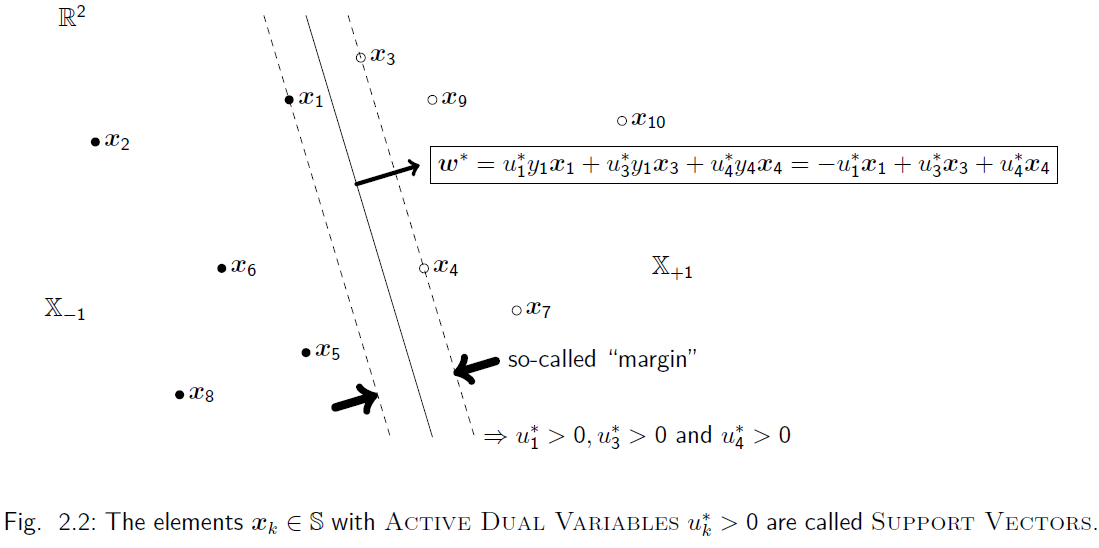
\includegraphics[width = \columnwidth]{geometric_int_svm}
	\paragraph{Discussion}
	\begin{itemize}
		\item Exists only if $\mathbb{S} $ \textbf{Linearly Separable}
		\item $w_0 \neq 0$ no (straightforward) iterative solution available
		\item if \textbf{Linearly Inseperable} method generalized by slack variables for controlled violation of constraints 
	\end{itemize}
$\rightarrow$ instead of $\smash{\displaystyle\min_{\mathbf{w}}}\frac{1}{2}\mathbf{w^Tw}$ s.t. $ y_k\mathbf{w^Tx}_k\geq1$ we get\\ $\smash{\displaystyle\min_{\mathbf{w},\epsilon}}\frac{1}{2}\mathbf{w^Tw} +\rho\sum_{k=1}^{M}\epsilon_k$ s.t.$ y_k\mathbf{w^Tx}_k\geq1-\epsilon_k, \forall k,\vec{\epsilon},\rho\geq0$
	
\end{sectionbox}

\begin{sectionbox}
	\subsection{Kernel Trick}
	\textbf{Linear Hypothesis Test} often not sufficient$\rightarrow$ \textbf{Kernel Trick}: Generalize linear methods to non-linear approximation of seperating surfaces $(\{x|\log R(\mathbf{x})=c\})$ \\
	Basic Idea: Transfer problem statement into higher-dimensional space(without introducing additional degrees of freedom) by \textbf{Feature Map} $\varphi: \mathbb{S}\rightarrow\mathbb{S}_{\varphi}$
	\\ 
 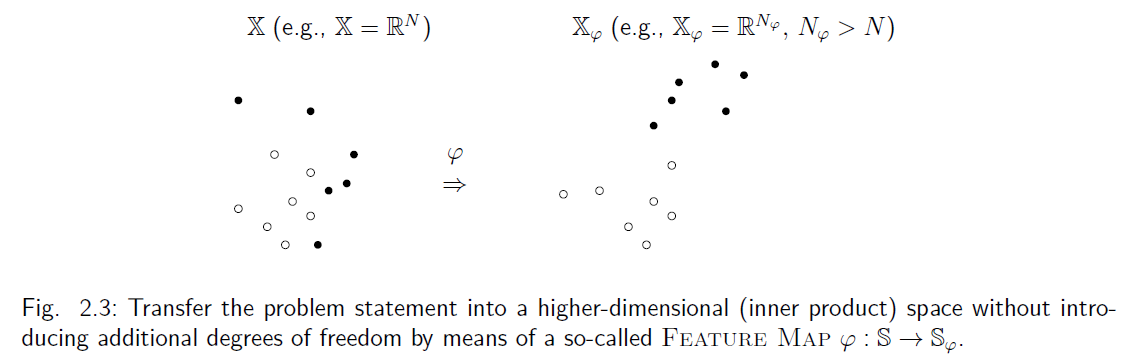
\includegraphics[width = \columnwidth]{kernel_trick} \\
 Construction of Linear Test in $\mathbb{R}^3$ correspondes to Non-Linear Test in $\mathbb{R}^2$\\
 $\boxed{T:\mathbb{R}^3\rightarrow\{-1,+1\},\varphi(\mathbf{x})\mapsto \begin{cases} +1 ;&\mathbf{w}_{\varphi}^T\varphi(\mathbf{x})\geq0\\
 -1;&otherwise \end{cases}}$ \\
	Linear kernel in $\mathbb{X}_\varphi$ represents nonlinear kernel in $\mathbb{X} \rightarrow$ choose g(.,.) directly instead of finding transformation $\varphi$  \\
	$\boxed{\langle\varphi(\mathbf{x}),\varphi(\mathbf{y})\rangle=:g(\mathbf{x,y})}$ \\

	In Optimization Problem and resulting Dual Function and Variables \\replace $\mathbf{x}$ by $\varphi(\mathbf{x}_k)$ $\rightarrow$ Dual OP: $\smash{\displaystyle\max_{\mathbf{u}\geq0}}\{-\mathbf{u^TYGYu +1^Tu}\}\\$ \\
	Kernel Matrix G = $\begin{bmatrix}
		g(\mathbf{x_1,x_2}) &\cdots& g(\mathbf{x_1,x_M}) \\
		\vdots&&\vdots \\
		g(\mathbf{x_M,x_1}) &\cdots& g(\mathbf{x_M,x_M}) 
	\end{bmatrix} \in \mathbb{R}^{MxM}$ \\
	After applying \textbf{Kernel Trick}: OP and Nonlinear Test T only based on Kernel Function g, transformation $\varphi$ becomes obsolete\\
	Hypothesis Test(nonlinear): $\boxed{T:\mathbf{x}\mapsto sign(\sum_{k=1}^{M}u_k^*y_kg(\mathbf{x_k,x}))}$\\

\end{sectionbox}
\begin{sectionbox}
	\paragraph{Possible Kernels for Kernel Trick}
	Linear Kernel: $g_{lin}(\mathbf{x},\mathbf{x}_k)=\mathbf{x}_k^T\mathbf{x}$\\
	Polynomial Kernel:$g_{poly}(\mathbf{x},\mathbf{x}_k)=(\mathbf{x}_k^T\mathbf{x}+1)^d$\\
	Sigmoid Kernel: $g_{sigm}(\mathbf{x},\mathbf{x}_k)=\tanh(\beta(\mathbf{x_k^Tx})+w_0)$ \\
	Radial Kernel: $g_{rbf}(\mathbf{x},\mathbf{x}_k)=\exp(-\frac{1}{2\sigma^2}\norm{\mathbf{x-x_k}}_2^2)$

 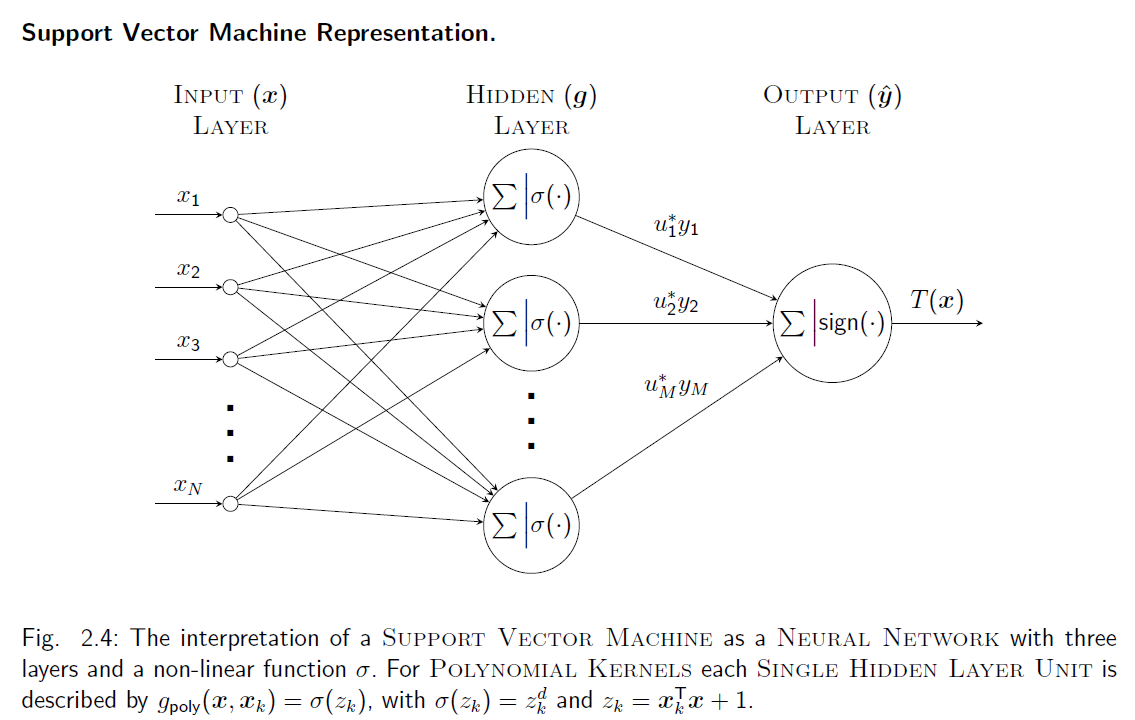
\includegraphics[width = \columnwidth]{svm_as_nn}
\end{sectionbox}	